% GNUPLOT: LaTeX picture with Postscript
\begingroup
  \makeatletter
  \providecommand\color[2][]{%
    \GenericError{(gnuplot) \space\space\space\@spaces}{%
      Package color not loaded in conjunction with
      terminal option `colourtext'%
    }{See the gnuplot documentation for explanation.%
    }{Either use 'blacktext' in gnuplot or load the package
      color.sty in LaTeX.}%
    \renewcommand\color[2][]{}%
  }%
  \providecommand\includegraphics[2][]{%
    \GenericError{(gnuplot) \space\space\space\@spaces}{%
      Package graphicx or graphics not loaded%
    }{See the gnuplot documentation for explanation.%
    }{The gnuplot epslatex terminal needs graphicx.sty or graphics.sty.}%
    \renewcommand\includegraphics[2][]{}%
  }%
  \providecommand\rotatebox[2]{#2}%
  \@ifundefined{ifGPcolor}{%
    \newif\ifGPcolor
    \GPcolortrue
  }{}%
  \@ifundefined{ifGPblacktext}{%
    \newif\ifGPblacktext
    \GPblacktexttrue
  }{}%
  % define a \g@addto@macro without @ in the name:
  \let\gplgaddtomacro\g@addto@macro
  % define empty templates for all commands taking text:
  \gdef\gplbacktext{}%
  \gdef\gplfronttext{}%
  \makeatother
  \ifGPblacktext
    % no textcolor at all
    \def\colorrgb#1{}%
    \def\colorgray#1{}%
  \else
    % gray or color?
    \ifGPcolor
      \def\colorrgb#1{\color[rgb]{#1}}%
      \def\colorgray#1{\color[gray]{#1}}%
      \expandafter\def\csname LTw\endcsname{\color{white}}%
      \expandafter\def\csname LTb\endcsname{\color{black}}%
      \expandafter\def\csname LTa\endcsname{\color{black}}%
      \expandafter\def\csname LT0\endcsname{\color[rgb]{1,0,0}}%
      \expandafter\def\csname LT1\endcsname{\color[rgb]{0,1,0}}%
      \expandafter\def\csname LT2\endcsname{\color[rgb]{0,0,1}}%
      \expandafter\def\csname LT3\endcsname{\color[rgb]{1,0,1}}%
      \expandafter\def\csname LT4\endcsname{\color[rgb]{0,1,1}}%
      \expandafter\def\csname LT5\endcsname{\color[rgb]{1,1,0}}%
      \expandafter\def\csname LT6\endcsname{\color[rgb]{0,0,0}}%
      \expandafter\def\csname LT7\endcsname{\color[rgb]{1,0.3,0}}%
      \expandafter\def\csname LT8\endcsname{\color[rgb]{0.5,0.5,0.5}}%
    \else
      % gray
      \def\colorrgb#1{\color{black}}%
      \def\colorgray#1{\color[gray]{#1}}%
      \expandafter\def\csname LTw\endcsname{\color{white}}%
      \expandafter\def\csname LTb\endcsname{\color{black}}%
      \expandafter\def\csname LTa\endcsname{\color{black}}%
      \expandafter\def\csname LT0\endcsname{\color{black}}%
      \expandafter\def\csname LT1\endcsname{\color{black}}%
      \expandafter\def\csname LT2\endcsname{\color{black}}%
      \expandafter\def\csname LT3\endcsname{\color{black}}%
      \expandafter\def\csname LT4\endcsname{\color{black}}%
      \expandafter\def\csname LT5\endcsname{\color{black}}%
      \expandafter\def\csname LT6\endcsname{\color{black}}%
      \expandafter\def\csname LT7\endcsname{\color{black}}%
      \expandafter\def\csname LT8\endcsname{\color{black}}%
    \fi
  \fi
    \setlength{\unitlength}{0.0500bp}%
    \ifx\gptboxheight\undefined%
      \newlength{\gptboxheight}%
      \newlength{\gptboxwidth}%
      \newsavebox{\gptboxtext}%
    \fi%
    \setlength{\fboxrule}{0.5pt}%
    \setlength{\fboxsep}{1pt}%
\begin{picture}(10080.00,4320.00)%
    \gplgaddtomacro\gplbacktext{%
      \csname LTb\endcsname%
      \put(946,704){\makebox(0,0)[r]{\strut{}$-1.5$}}%
      \put(946,1263){\makebox(0,0)[r]{\strut{}$-1$}}%
      \put(946,1821){\makebox(0,0)[r]{\strut{}$-0.5$}}%
      \put(946,2380){\makebox(0,0)[r]{\strut{}$0$}}%
      \put(946,2938){\makebox(0,0)[r]{\strut{}$0.5$}}%
      \put(946,3497){\makebox(0,0)[r]{\strut{}$1$}}%
      \put(946,4055){\makebox(0,0)[r]{\strut{}$1.5$}}%
      \put(1078,484){\makebox(0,0){\strut{}$-5$}}%
      \put(1435,484){\makebox(0,0){\strut{}$-4$}}%
      \put(1791,484){\makebox(0,0){\strut{}$-3$}}%
      \put(2148,484){\makebox(0,0){\strut{}$-2$}}%
      \put(2504,484){\makebox(0,0){\strut{}$-1$}}%
      \put(2861,484){\makebox(0,0){\strut{}$0$}}%
      \put(3217,484){\makebox(0,0){\strut{}$1$}}%
      \put(3574,484){\makebox(0,0){\strut{}$2$}}%
      \put(3930,484){\makebox(0,0){\strut{}$3$}}%
      \put(4287,484){\makebox(0,0){\strut{}$4$}}%
      \put(4643,484){\makebox(0,0){\strut{}$5$}}%
    }%
    \gplgaddtomacro\gplfronttext{%
      \csname LTb\endcsname%
      \put(176,2379){\rotatebox{-270}{\makebox(0,0){\strut{}p, a.u.}}}%
      \put(2860,154){\makebox(0,0){\strut{}q, a.u}}%
      \csname LTb\endcsname%
      \put(2273,2790){\makebox(0,0)[r]{\strut{}$p_1 : q_1$}}%
      \csname LTb\endcsname%
      \put(2273,2570){\makebox(0,0)[r]{\strut{}$p_2 : q_2$}}%
      \csname LTb\endcsname%
      \put(2273,2350){\makebox(0,0)[r]{\strut{}$p_3 : q_3$}}%
    }%
    \gplgaddtomacro\gplbacktext{%
      \csname LTb\endcsname%
      \put(5986,704){\makebox(0,0)[r]{\strut{}$-1.5$}}%
      \put(5986,1263){\makebox(0,0)[r]{\strut{}$-1$}}%
      \put(5986,1821){\makebox(0,0)[r]{\strut{}$-0.5$}}%
      \put(5986,2380){\makebox(0,0)[r]{\strut{}$0$}}%
      \put(5986,2938){\makebox(0,0)[r]{\strut{}$0.5$}}%
      \put(5986,3497){\makebox(0,0)[r]{\strut{}$1$}}%
      \put(5986,4055){\makebox(0,0)[r]{\strut{}$1.5$}}%
      \put(6118,484){\makebox(0,0){\strut{}$-5$}}%
      \put(6475,484){\makebox(0,0){\strut{}$-4$}}%
      \put(6831,484){\makebox(0,0){\strut{}$-3$}}%
      \put(7188,484){\makebox(0,0){\strut{}$-2$}}%
      \put(7544,484){\makebox(0,0){\strut{}$-1$}}%
      \put(7901,484){\makebox(0,0){\strut{}$0$}}%
      \put(8257,484){\makebox(0,0){\strut{}$1$}}%
      \put(8614,484){\makebox(0,0){\strut{}$2$}}%
      \put(8970,484){\makebox(0,0){\strut{}$3$}}%
      \put(9327,484){\makebox(0,0){\strut{}$4$}}%
      \put(9683,484){\makebox(0,0){\strut{}$5$}}%
    }%
    \gplgaddtomacro\gplfronttext{%
      \csname LTb\endcsname%
      \put(5216,2379){\rotatebox{-270}{\makebox(0,0){\strut{}p, a.u.}}}%
      \put(7900,154){\makebox(0,0){\strut{}q, a.u}}%
      \csname LTb\endcsname%
      \put(7313,2350){\makebox(0,0)[r]{\strut{}$\langle p\rangle : \langle q\rangle$}}%
    }%
    \gplbacktext
    \put(0,0){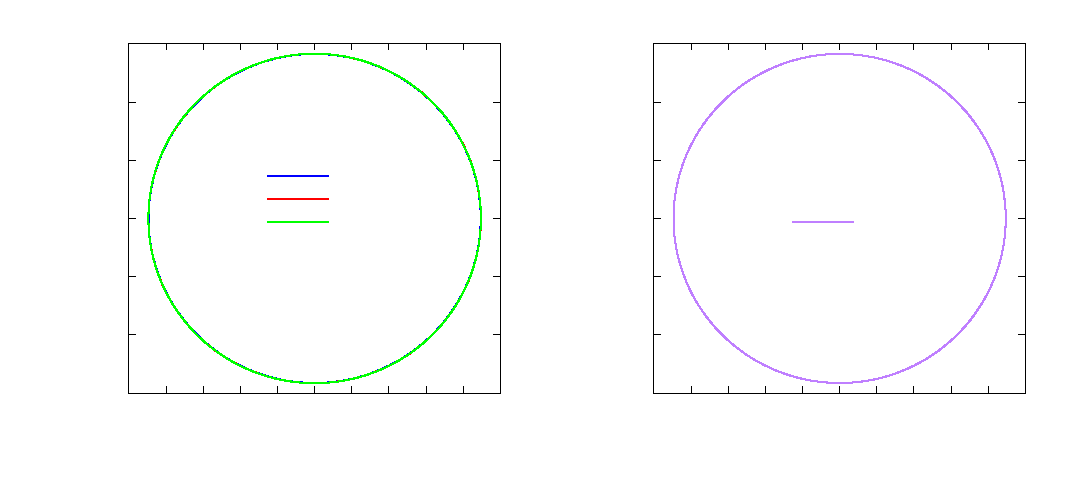
\includegraphics{results-gnuplottex-fig19}}%
    \gplfronttext
  \end{picture}%
\endgroup
